\documentclass[a4paper 12pts]{article}
\usepackage[utf8]{inputenc}
\usepackage[T1]{fontenc}
\usepackage[francais]{babel}
\usepackage{graphicx}


\title{Rapport de Projet : iRover}

%mettez vos noms svp!!!!!!

\author{R. Joachim CLAYTON}
\author{Geoffrey DESBROSSES}

\begin{document}

\maketitle


\begin{figure}[h]
   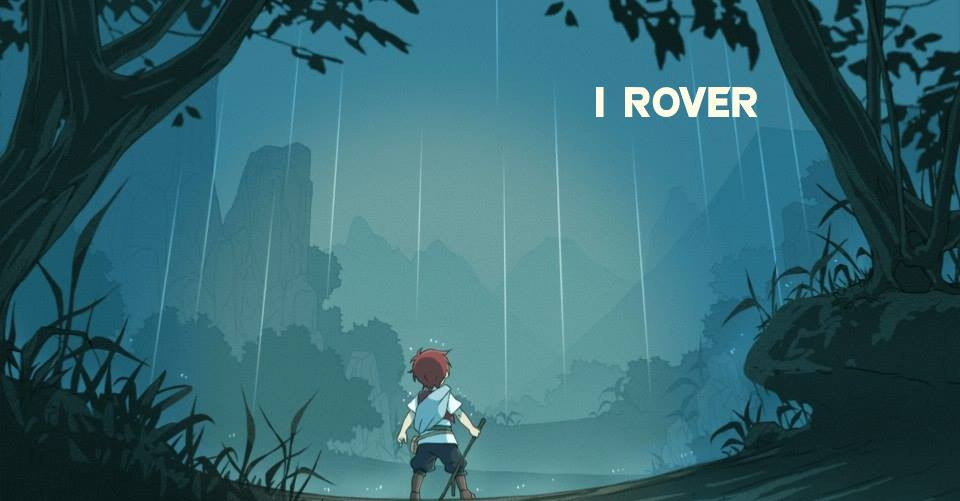
\includegraphics[width=350pt]{Illustration/proj_irover.jpg}
	\caption{iRover, l'histoire d'un héros qu'on appellait robot}
\end{figure}



\newpage


\renewcommand{\contentsname}{Sommaire} 
\tableofcontents

\newpage








\section{Rapport de Projet}


\vspace{2cm}



\subsection{Introduction}

\vspace{1 cm}


Le projet a pour objectif la création d'une application graphique où un petit personnage (robot) réaliserait une tache particulière.\\
Pour cela nous avons imaginé un scénario de mini jeu semblable au jeux en deux dimensions où notre robot prendrait la forme d'un héros sans peur et sans reproche.\\
L'autre aspect de ce projet est de pousser notre groupe à utiliser, comprendre et intégrer les autotools.
\vspace{1 cm}


\subsection{Membre du groupe et tâches de chacun}
\vspace{1 cm}



\vspace{1 cm}

\begin{tabular}{| c | p{6cm} | c |}
\hline
\textbf{Responsable} & \textbf{Tâche} & \textbf {Description} \\
\hline
Clément Bauchet & Création graphique & La création de l'environnement graphiques et des images \\					
& Parsing de la carte & L'interprétation entre les objets graphiques et les objets C++\\					
\hline				
Geoffrey Desbrosses & Création des objets & Création de chaque objet de l'application et de leurs actions\\
& Documentation du code source & Gestion de la documentation Doxygen \\ 
\hline
& IHM & Interface utilisateur de l'application. \\
\hline
Jean-Christophe Guerin & IA  & Définitions des algorithmes de pathfinding de déplacement et de découverte\\	
\hline
Joachim Clayton & Documentation utilisateur & Redaction de la documentation utilisateur \\                 
\end{tabular}





\newpage
\section{Définition de la Carte}


%partie de Clément

%mettre une petite introduction et parlez de vos parties


\newpage
%partie Geoffrey

\section{Définition des objets}
La définition des objets comprend la création de tous les objets Personnage, Coffre, Clef, Arme\ldots et toutes les actions entre ces objets.

\subsection{Les objets existants}
Le robot possède une fonction pour se déplacer et modifier ses coordonnées. Il possède également une méthode combattre propre à notre sujet. Des actuateurs arme et armure ont été implémentés. Le robot peut intéragir avec d'autres objets tels que les ennemis, les clefs ou les coffres. Deux types d'armes ont également été créé (bazooka et mine) et les classes Arme et Armures permettent d'implémenter facilement de nouvelles armes et armures ayant leurs propres caractéristiques.

\subsection{Les objets manquant}
Le robot ne possède pas de senseur. L'idée était d'implémenter un scanner qui pouvait scanner une carte et savoir quels étaient les cases du terrain où le robot pouvait aller. Aucun type d'armure n'a été implémenté, cependant les personnages peuvent tout de même avoir une armure par défaut avec une robustesse et un nom. Ainsi ça ne modifie pas le comportement des personnages.

\subsection{gestion des évênements}
Certains objets peuvent intéragir entre eux, par exemple la mine peut exploser au contact d'un ennemi, deux personnages peuvent s'affronter, le robot peut ramasser des clefs et ouvrir des coffres. Cependant, ces actions ne sont pas visibles sur l'interface graphique, excepté le déplacement du robot.

\section{IHM}


\newpage
\section{IA}

%partie JC
%mettre une petite introduction et parlez de vos parties

\subsection{path finding}
\subsection{découverte de la carte}


\newpage
\section{Problèmes rencontrer}


\section{Conclusion}



\end{document}

